\begin{frame}
  \frametitle{Prediction using Random Error with Nuclide Masses}
  \begin{minipage}{0.49\textwidth}
    \begin{figure}
      \centering
      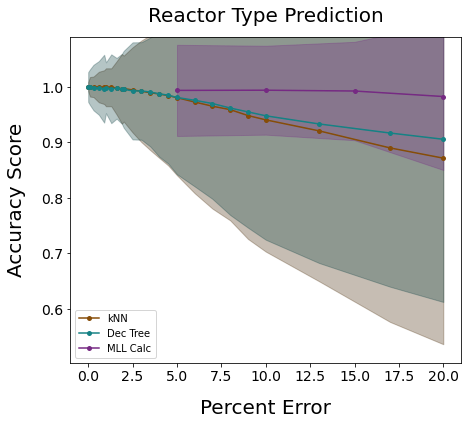
\includegraphics[width=\linewidth]{./figures/randerr_compare_nuc29_rxtr.png}
      \caption{caption}
    \end{figure}
  \end{minipage}%
  \hfill
  \begin{minipage}{0.49\textwidth}
    \begin{figure}
      \centering
      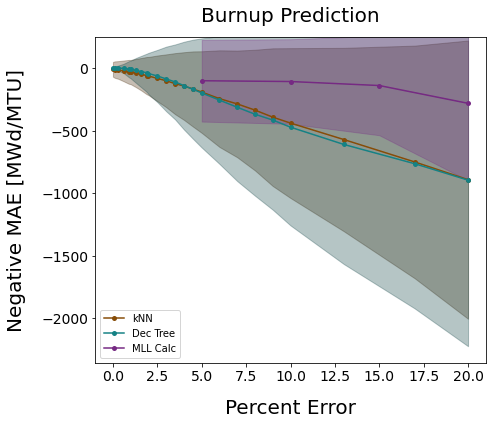
\includegraphics[width=\linewidth]{./figures/randerr_compare_nuc29_burn.png}
      \caption{caption}
    \end{figure}
  \end{minipage}%
\end{frame}

\begin{frame}
  \frametitle{Prediction using Random Error with Nuclide Masses}
  \begin{minipage}{0.49\textwidth}
    \begin{figure}
      \centering
      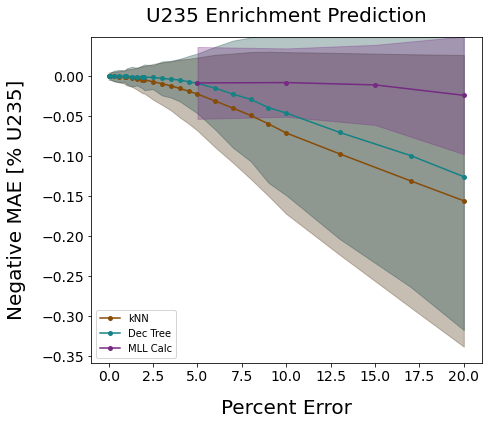
\includegraphics[width=\linewidth]{./figures/randerr_compare_nuc29_enri.png}
      \caption{caption}
    \end{figure}
  \end{minipage}%
  \hfill
  \begin{minipage}{0.49\textwidth}
    \begin{figure}
      \centering
      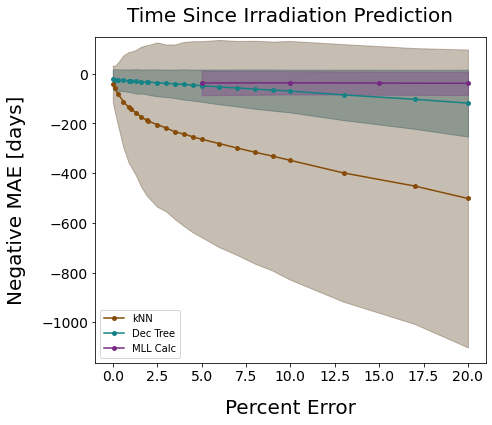
\includegraphics[width=\linewidth]{./figures/randerr_compare_nuc29_cool.png}
      \caption{caption}
    \end{figure}
  \end{minipage}%
\end{frame}
\begin{frame}
  \frametitle{SFCOMPO}
  \begin{figure}
    \centering
    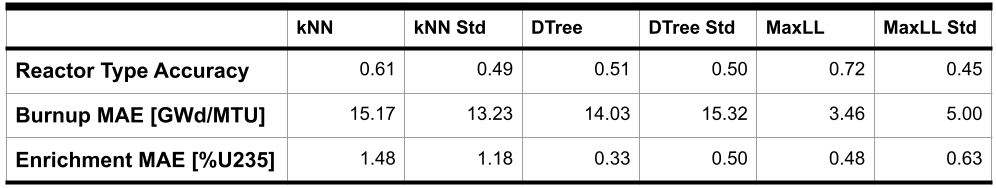
\includegraphics[width=\textwidth]{./figures/sfcompo_pred_results.png}
    \caption{caption}
  \end{figure}
\end{frame}
